\chapter{uForth Editor}
\label{chap:fortheditor}
In diesem Kapitel wird beschrieben, wie das Framework Xtext funktioniert und wie es verwendet wurde, um Feature wie Syntax Highlighting, eine Outline und Dokumentations Popups für den Forth Editor zu implementieren.

\section{Xtext Implementation des uForth Editor}
Xtext ermöglicht es, das Grundgerüst einer Entwicklungsumgebung zu generieren. Dafür verwendet Xtext eine Extended Backus-Naur Form (EBNF) ähnliche Grammatik. Aus dieser Grammatik wird dann ein ANTLR-Parser und Klassen, welche für den Editor benötigt werden, generiert. Um Xtext zu konfigurieren wird die dependency injection (DI) Library, Guice von Google verwendet. Mit Guice können viele Teile von Xtext in einem zentralen Modul mittels DI ersetzt werden.\\
Da Forth kein monolithischen Compiler und somit keine statische Grammatik besitzt, kann keine Grammatik für Xtext geschrieben werden, welche die gesammte Forth Sprache beschreibt. Es wurde deshalb eine Xtext Grammtik verwendet, welche ungefähr der folgenden EBNF Grammtik entspricht.

\begin{verbatim}
instructoin = create | function | word;
function = ':', identifier, { Word }, ';';
create = 'create', identifier, { literal ',' };
word = identifier;
\end{verbatim}

Wobei die \verb!identifier! Regel alle gültigen Forth Identifier beschreibt und die \verb!literal! Regel alle gültigen Integer und Double Werte beschreibt.
\\
Der daraus generierte Parser kann alle vom LCC generierten Forth Files parsen und reicht somit für die Entwicklungsumgebung aus. 

\newpage
\section{uForth Editor}
Der Editor unterstützt Syntax Highligting für vordefinierte Forth Wörter, Literals und Kommentare. Die Wörter werden in drei Gruppen unterteilt. Stack-, Memory- und Arithmetische-Wörter. Alle Gruppen haben eine andere Farbe, welche in der uForth Preference Page geändert werden kann. In folgender Abbildung \ref{fig:fortheditor} ist der uForth Editor zu sehen.


\begin{figure}[H]
	\centering
		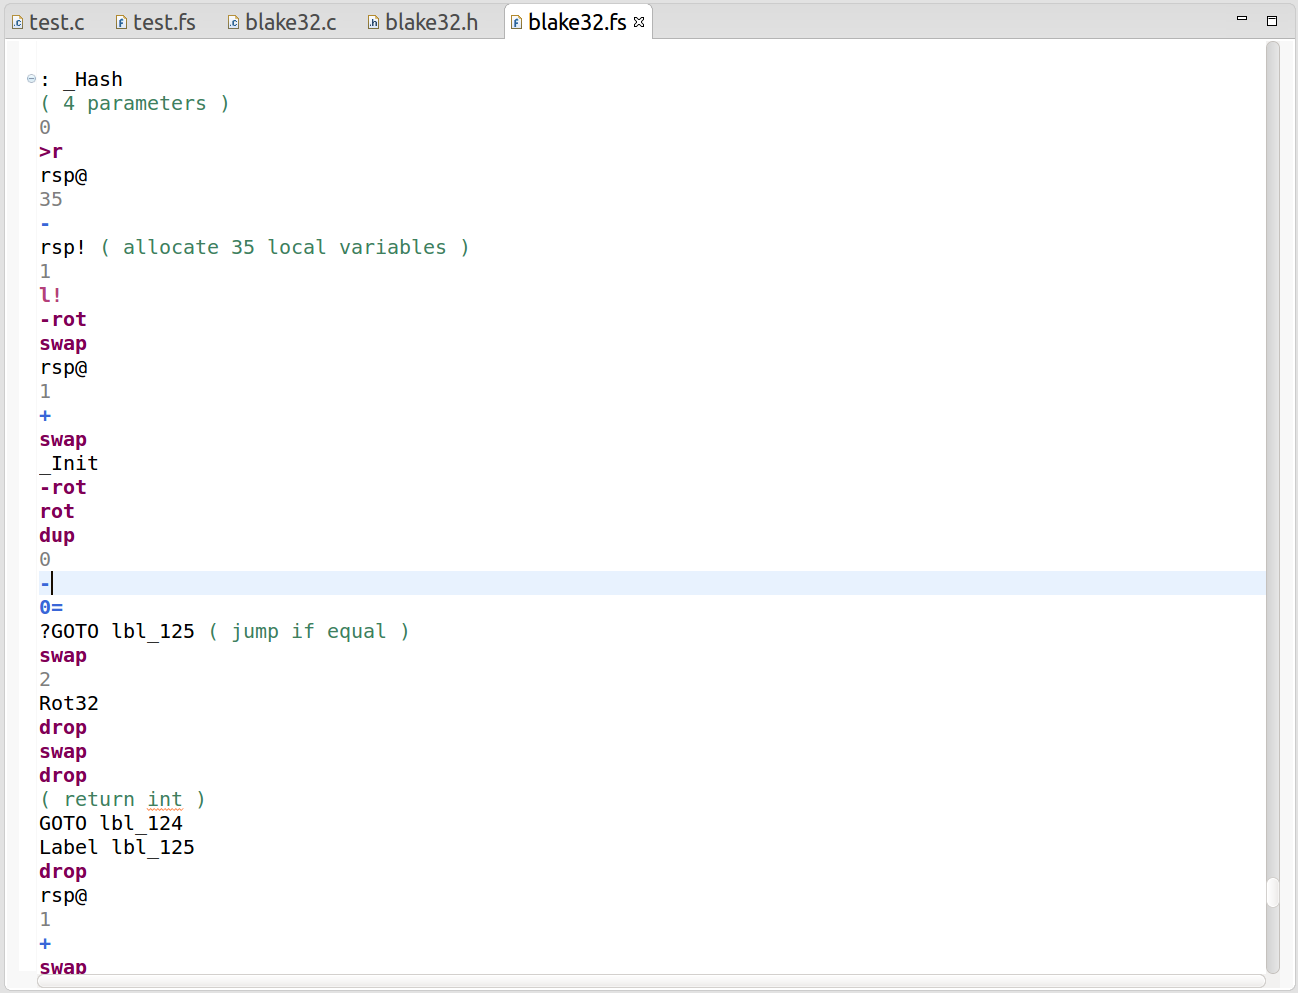
\includegraphics[scale=0.4]{fortheditor/fortheditor.png}
		\caption{uForth Editor, welcher vorallem für den Debugger verwendet wird.}
		\captionsetup{margin=0cm,font={footnotesize}}
		\label{fig:fortheditor}
\end{figure}

\newpage

\subsection{Wörter Dokumentation}
Eine Dokumentation wurde für uForth spezifischen Wörter als Popup implementiert. Die Dokumentation wird dafür aus einer Textdatei gelesen. In folgender Abbildung \ref{fig:docpopup} ist eine Popup Dokumentation zu dem Wort \verb!label! zu sehen.

\begin{figure}[H]
	\centering
		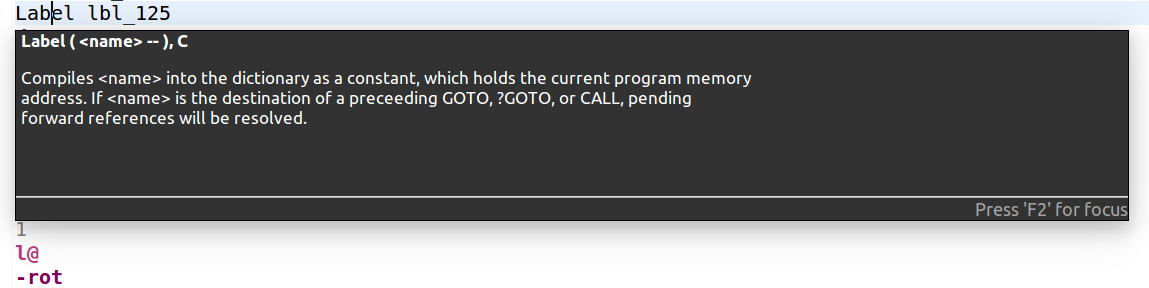
\includegraphics[scale=0.4]{fortheditor/doc.png}
		\caption{Popup Dokumentation zu dem Wort label. Die Dokumentation wird angezeigt, falls der Cursor sich über einem Wort befindet, für welches eine Dokumentation verfügbar ist.}
		\captionsetup{margin=0cm,font={footnotesize}}
		\label{fig:docpopup}
\end{figure}

\subsection{Editor Outline}
Für den Editor steht zudem eine Outline zur Verfügung. Die Outline gliedert das Forth File nach den von der Grammatik spezifizierten Regeln. Für den uForth Editor bedeutet das, dass das File nach Funktionen und Wörtern gegliedert wird.

\begin{figure}[H]
	\centering
		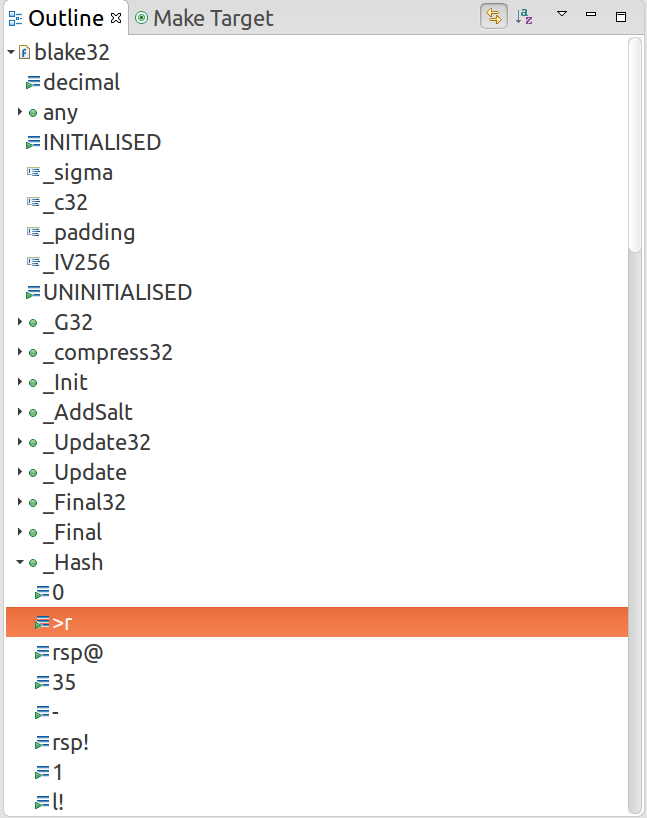
\includegraphics[scale=0.3]{fortheditor/outline.png}
		\caption{Outline zu einem Forth File. Die Outline gliedert das File in Funktionen und Wörter.}
		\captionsetup{margin=0cm,font={footnotesize}}
		\label{fig:outlineeditor}
\end{figure}

